% Created by tikzDevice version 0.12.6 on 2024-03-14 07:38:59
% !TEX encoding = UTF-8 Unicode
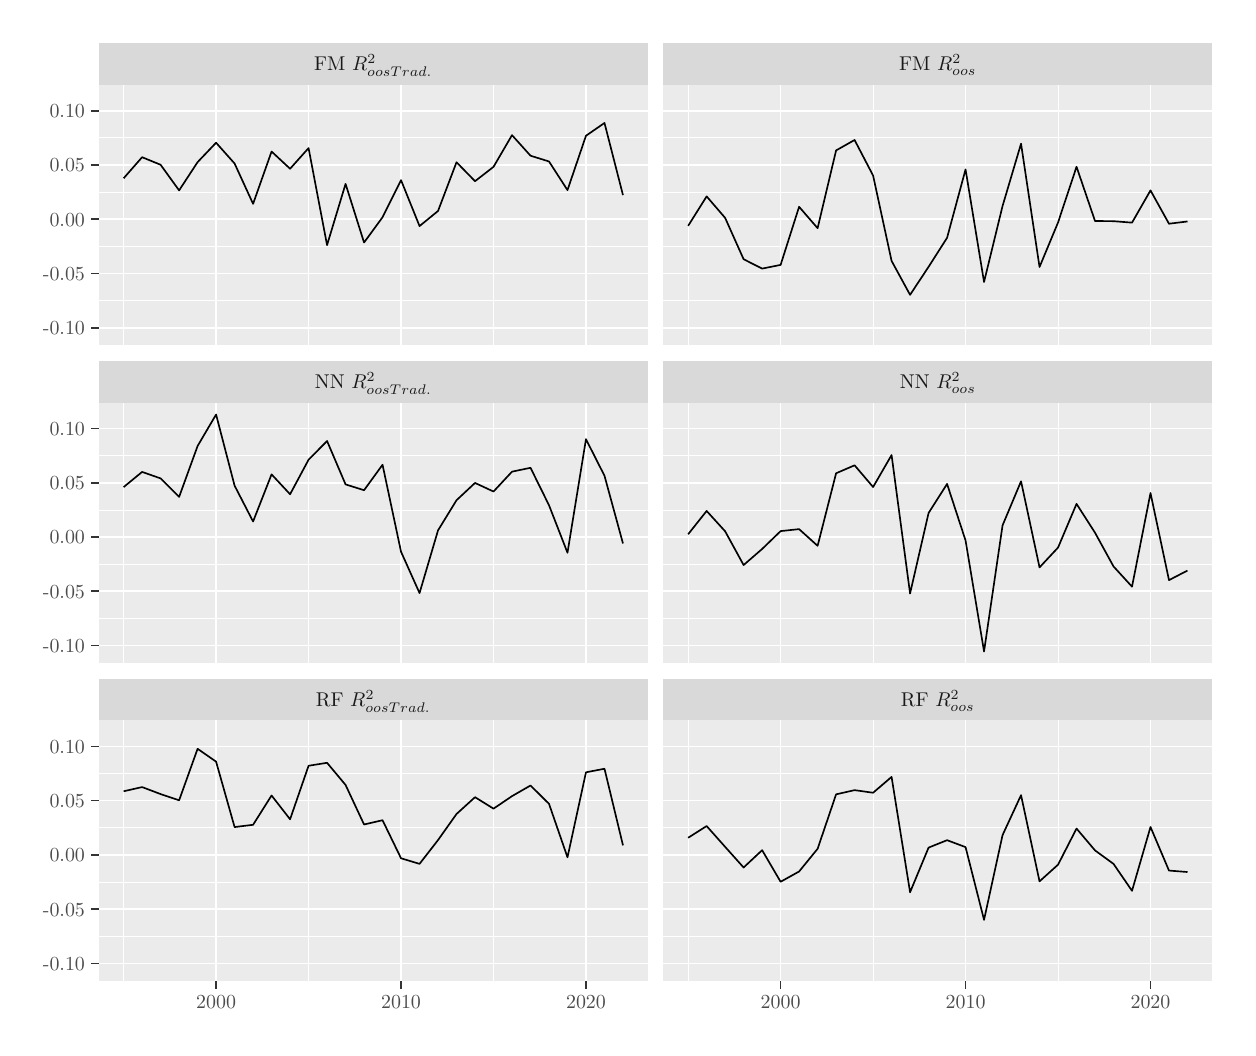
\begin{tikzpicture}[x=1pt,y=1pt]
\definecolor{fillColor}{RGB}{255,255,255}
\path[use as bounding box,fill=fillColor,fill opacity=0.00] (0,0) rectangle (433.62,361.35);
\begin{scope}
\path[clip] (  0.00,  0.00) rectangle (433.62,361.35);
\definecolor{drawColor}{RGB}{255,255,255}
\definecolor{fillColor}{RGB}{255,255,255}

\path[draw=drawColor,line width= 0.6pt,line join=round,line cap=round,fill=fillColor] (  0.00,  0.00) rectangle (433.62,361.35);
\end{scope}
\begin{scope}
\path[clip] ( 25.65,246.50) rectangle (224.13,340.69);
\definecolor{fillColor}{gray}{0.92}

\path[fill=fillColor] ( 25.65,246.50) rectangle (224.13,340.69);
\definecolor{drawColor}{RGB}{255,255,255}

\path[draw=drawColor,line width= 0.3pt,line join=round] ( 25.65,262.73) --
	(224.13,262.73);

\path[draw=drawColor,line width= 0.3pt,line join=round] ( 25.65,282.33) --
	(224.13,282.33);

\path[draw=drawColor,line width= 0.3pt,line join=round] ( 25.65,301.93) --
	(224.13,301.93);

\path[draw=drawColor,line width= 0.3pt,line join=round] ( 25.65,321.53) --
	(224.13,321.53);

\path[draw=drawColor,line width= 0.3pt,line join=round] ( 34.67,246.50) --
	( 34.67,340.69);

\path[draw=drawColor,line width= 0.3pt,line join=round] (101.50,246.50) --
	(101.50,340.69);

\path[draw=drawColor,line width= 0.3pt,line join=round] (168.33,246.50) --
	(168.33,340.69);

\path[draw=drawColor,line width= 0.6pt,line join=round] ( 25.65,252.92) --
	(224.13,252.92);

\path[draw=drawColor,line width= 0.6pt,line join=round] ( 25.65,272.53) --
	(224.13,272.53);

\path[draw=drawColor,line width= 0.6pt,line join=round] ( 25.65,292.13) --
	(224.13,292.13);

\path[draw=drawColor,line width= 0.6pt,line join=round] ( 25.65,311.73) --
	(224.13,311.73);

\path[draw=drawColor,line width= 0.6pt,line join=round] ( 25.65,331.33) --
	(224.13,331.33);

\path[draw=drawColor,line width= 0.6pt,line join=round] ( 68.08,246.50) --
	( 68.08,340.69);

\path[draw=drawColor,line width= 0.6pt,line join=round] (134.91,246.50) --
	(134.91,340.69);

\path[draw=drawColor,line width= 0.6pt,line join=round] (201.74,246.50) --
	(201.74,340.69);
\definecolor{drawColor}{RGB}{0,0,0}

\path[draw=drawColor,line width= 0.6pt,line join=round] ( 34.67,306.92) --
	( 41.35,314.54) --
	( 48.03,311.81) --
	( 54.72,302.55) --
	( 61.40,312.76) --
	( 68.08,319.77) --
	( 74.77,312.26) --
	( 81.45,297.68) --
	( 88.13,316.59) --
	( 94.82,310.37) --
	(101.50,317.84) --
	(108.18,282.78) --
	(114.87,304.90) --
	(121.55,283.71) --
	(128.23,292.84) --
	(134.91,306.26) --
	(141.60,289.65) --
	(148.28,295.11) --
	(154.96,312.72) --
	(161.65,305.87) --
	(168.33,311.06) --
	(175.01,322.51) --
	(181.70,315.08) --
	(188.38,313.00) --
	(195.06,302.65) --
	(201.74,322.29) --
	(208.43,326.91) --
	(215.11,300.85);
\end{scope}
\begin{scope}
\path[clip] ( 25.65,131.66) rectangle (224.13,225.84);
\definecolor{fillColor}{gray}{0.92}

\path[fill=fillColor] ( 25.65,131.66) rectangle (224.13,225.84);
\definecolor{drawColor}{RGB}{255,255,255}

\path[draw=drawColor,line width= 0.3pt,line join=round] ( 25.65,147.88) --
	(224.13,147.88);

\path[draw=drawColor,line width= 0.3pt,line join=round] ( 25.65,167.48) --
	(224.13,167.48);

\path[draw=drawColor,line width= 0.3pt,line join=round] ( 25.65,187.08) --
	(224.13,187.08);

\path[draw=drawColor,line width= 0.3pt,line join=round] ( 25.65,206.68) --
	(224.13,206.68);

\path[draw=drawColor,line width= 0.3pt,line join=round] ( 34.67,131.66) --
	( 34.67,225.84);

\path[draw=drawColor,line width= 0.3pt,line join=round] (101.50,131.66) --
	(101.50,225.84);

\path[draw=drawColor,line width= 0.3pt,line join=round] (168.33,131.66) --
	(168.33,225.84);

\path[draw=drawColor,line width= 0.6pt,line join=round] ( 25.65,138.08) --
	(224.13,138.08);

\path[draw=drawColor,line width= 0.6pt,line join=round] ( 25.65,157.68) --
	(224.13,157.68);

\path[draw=drawColor,line width= 0.6pt,line join=round] ( 25.65,177.28) --
	(224.13,177.28);

\path[draw=drawColor,line width= 0.6pt,line join=round] ( 25.65,196.88) --
	(224.13,196.88);

\path[draw=drawColor,line width= 0.6pt,line join=round] ( 25.65,216.49) --
	(224.13,216.49);

\path[draw=drawColor,line width= 0.6pt,line join=round] ( 68.08,131.66) --
	( 68.08,225.84);

\path[draw=drawColor,line width= 0.6pt,line join=round] (134.91,131.66) --
	(134.91,225.84);

\path[draw=drawColor,line width= 0.6pt,line join=round] (201.74,131.66) --
	(201.74,225.84);
\definecolor{drawColor}{RGB}{0,0,0}

\path[draw=drawColor,line width= 0.6pt,line join=round] ( 34.67,195.33) --
	( 41.35,200.82) --
	( 48.03,198.48) --
	( 54.72,191.78) --
	( 61.40,210.18) --
	( 68.08,221.56) --
	( 74.77,195.85) --
	( 81.45,182.90) --
	( 88.13,199.93) --
	( 94.82,192.75) --
	(101.50,205.22) --
	(108.18,211.99) --
	(114.87,196.31) --
	(121.55,194.21) --
	(128.23,203.41) --
	(134.91,171.98) --
	(141.60,157.04) --
	(148.28,179.70) --
	(154.96,190.59) --
	(161.65,196.84) --
	(168.33,193.73) --
	(175.01,200.91) --
	(181.70,202.31) --
	(188.38,188.78) --
	(195.06,171.61) --
	(201.74,212.64) --
	(208.43,199.43) --
	(215.11,174.97);
\end{scope}
\begin{scope}
\path[clip] ( 25.65, 16.81) rectangle (224.13,111.00);
\definecolor{fillColor}{gray}{0.92}

\path[fill=fillColor] ( 25.65, 16.81) rectangle (224.13,111.00);
\definecolor{drawColor}{RGB}{255,255,255}

\path[draw=drawColor,line width= 0.3pt,line join=round] ( 25.65, 33.03) --
	(224.13, 33.03);

\path[draw=drawColor,line width= 0.3pt,line join=round] ( 25.65, 52.63) --
	(224.13, 52.63);

\path[draw=drawColor,line width= 0.3pt,line join=round] ( 25.65, 72.24) --
	(224.13, 72.24);

\path[draw=drawColor,line width= 0.3pt,line join=round] ( 25.65, 91.84) --
	(224.13, 91.84);

\path[draw=drawColor,line width= 0.3pt,line join=round] ( 34.67, 16.81) --
	( 34.67,111.00);

\path[draw=drawColor,line width= 0.3pt,line join=round] (101.50, 16.81) --
	(101.50,111.00);

\path[draw=drawColor,line width= 0.3pt,line join=round] (168.33, 16.81) --
	(168.33,111.00);

\path[draw=drawColor,line width= 0.6pt,line join=round] ( 25.65, 23.23) --
	(224.13, 23.23);

\path[draw=drawColor,line width= 0.6pt,line join=round] ( 25.65, 42.83) --
	(224.13, 42.83);

\path[draw=drawColor,line width= 0.6pt,line join=round] ( 25.65, 62.43) --
	(224.13, 62.43);

\path[draw=drawColor,line width= 0.6pt,line join=round] ( 25.65, 82.04) --
	(224.13, 82.04);

\path[draw=drawColor,line width= 0.6pt,line join=round] ( 25.65,101.64) --
	(224.13,101.64);

\path[draw=drawColor,line width= 0.6pt,line join=round] ( 68.08, 16.81) --
	( 68.08,111.00);

\path[draw=drawColor,line width= 0.6pt,line join=round] (134.91, 16.81) --
	(134.91,111.00);

\path[draw=drawColor,line width= 0.6pt,line join=round] (201.74, 16.81) --
	(201.74,111.00);
\definecolor{drawColor}{RGB}{0,0,0}

\path[draw=drawColor,line width= 0.6pt,line join=round] ( 34.67, 85.42) --
	( 41.35, 86.94) --
	( 48.03, 84.41) --
	( 54.72, 82.15) --
	( 61.40,100.77) --
	( 68.08, 96.13) --
	( 74.77, 72.49) --
	( 81.45, 73.31) --
	( 88.13, 83.90) --
	( 94.82, 75.30) --
	(101.50, 94.64) --
	(108.18, 95.71) --
	(114.87, 87.71) --
	(121.55, 73.42) --
	(128.23, 74.96) --
	(134.91, 61.21) --
	(141.60, 59.19) --
	(148.28, 67.79) --
	(154.96, 77.21) --
	(161.65, 83.29) --
	(168.33, 79.14) --
	(175.01, 83.66) --
	(181.70, 87.51) --
	(188.38, 80.89) --
	(195.06, 61.56) --
	(201.74, 92.28) --
	(208.43, 93.56) --
	(215.11, 65.89);
\end{scope}
\begin{scope}
\path[clip] (229.63,246.50) rectangle (428.12,340.69);
\definecolor{fillColor}{gray}{0.92}

\path[fill=fillColor] (229.63,246.50) rectangle (428.12,340.69);
\definecolor{drawColor}{RGB}{255,255,255}

\path[draw=drawColor,line width= 0.3pt,line join=round] (229.63,262.73) --
	(428.12,262.73);

\path[draw=drawColor,line width= 0.3pt,line join=round] (229.63,282.33) --
	(428.12,282.33);

\path[draw=drawColor,line width= 0.3pt,line join=round] (229.63,301.93) --
	(428.12,301.93);

\path[draw=drawColor,line width= 0.3pt,line join=round] (229.63,321.53) --
	(428.12,321.53);

\path[draw=drawColor,line width= 0.3pt,line join=round] (238.66,246.50) --
	(238.66,340.69);

\path[draw=drawColor,line width= 0.3pt,line join=round] (305.49,246.50) --
	(305.49,340.69);

\path[draw=drawColor,line width= 0.3pt,line join=round] (372.32,246.50) --
	(372.32,340.69);

\path[draw=drawColor,line width= 0.6pt,line join=round] (229.63,252.92) --
	(428.12,252.92);

\path[draw=drawColor,line width= 0.6pt,line join=round] (229.63,272.53) --
	(428.12,272.53);

\path[draw=drawColor,line width= 0.6pt,line join=round] (229.63,292.13) --
	(428.12,292.13);

\path[draw=drawColor,line width= 0.6pt,line join=round] (229.63,311.73) --
	(428.12,311.73);

\path[draw=drawColor,line width= 0.6pt,line join=round] (229.63,331.33) --
	(428.12,331.33);

\path[draw=drawColor,line width= 0.6pt,line join=round] (272.07,246.50) --
	(272.07,340.69);

\path[draw=drawColor,line width= 0.6pt,line join=round] (338.90,246.50) --
	(338.90,340.69);

\path[draw=drawColor,line width= 0.6pt,line join=round] (405.73,246.50) --
	(405.73,340.69);
\definecolor{drawColor}{RGB}{0,0,0}

\path[draw=drawColor,line width= 0.6pt,line join=round] (238.66,289.74) --
	(245.34,300.38) --
	(252.02,292.62) --
	(258.70,277.68) --
	(265.39,274.28) --
	(272.07,275.62) --
	(278.75,296.62) --
	(285.44,288.89) --
	(292.12,316.99) --
	(298.80,320.76) --
	(305.49,307.91) --
	(312.17,277.07) --
	(318.85,264.81) --
	(325.54,274.93) --
	(332.22,285.41) --
	(338.90,310.13) --
	(345.58,269.46) --
	(352.27,296.91) --
	(358.95,319.42) --
	(365.63,274.87) --
	(372.32,290.94) --
	(379.00,311.09) --
	(385.68,291.49) --
	(392.37,291.42) --
	(399.05,290.89) --
	(405.73,302.54) --
	(412.41,290.50) --
	(419.10,291.32);
\end{scope}
\begin{scope}
\path[clip] (229.63,131.66) rectangle (428.12,225.84);
\definecolor{fillColor}{gray}{0.92}

\path[fill=fillColor] (229.63,131.66) rectangle (428.12,225.84);
\definecolor{drawColor}{RGB}{255,255,255}

\path[draw=drawColor,line width= 0.3pt,line join=round] (229.63,147.88) --
	(428.12,147.88);

\path[draw=drawColor,line width= 0.3pt,line join=round] (229.63,167.48) --
	(428.12,167.48);

\path[draw=drawColor,line width= 0.3pt,line join=round] (229.63,187.08) --
	(428.12,187.08);

\path[draw=drawColor,line width= 0.3pt,line join=round] (229.63,206.68) --
	(428.12,206.68);

\path[draw=drawColor,line width= 0.3pt,line join=round] (238.66,131.66) --
	(238.66,225.84);

\path[draw=drawColor,line width= 0.3pt,line join=round] (305.49,131.66) --
	(305.49,225.84);

\path[draw=drawColor,line width= 0.3pt,line join=round] (372.32,131.66) --
	(372.32,225.84);

\path[draw=drawColor,line width= 0.6pt,line join=round] (229.63,138.08) --
	(428.12,138.08);

\path[draw=drawColor,line width= 0.6pt,line join=round] (229.63,157.68) --
	(428.12,157.68);

\path[draw=drawColor,line width= 0.6pt,line join=round] (229.63,177.28) --
	(428.12,177.28);

\path[draw=drawColor,line width= 0.6pt,line join=round] (229.63,196.88) --
	(428.12,196.88);

\path[draw=drawColor,line width= 0.6pt,line join=round] (229.63,216.49) --
	(428.12,216.49);

\path[draw=drawColor,line width= 0.6pt,line join=round] (272.07,131.66) --
	(272.07,225.84);

\path[draw=drawColor,line width= 0.6pt,line join=round] (338.90,131.66) --
	(338.90,225.84);

\path[draw=drawColor,line width= 0.6pt,line join=round] (405.73,131.66) --
	(405.73,225.84);
\definecolor{drawColor}{RGB}{0,0,0}

\path[draw=drawColor,line width= 0.6pt,line join=round] (238.66,178.30) --
	(245.34,186.71) --
	(252.02,179.37) --
	(258.70,167.17) --
	(265.39,172.97) --
	(272.07,179.43) --
	(278.75,180.15) --
	(285.44,174.11) --
	(292.12,200.33) --
	(298.80,203.21) --
	(305.49,195.36) --
	(312.17,206.91) --
	(318.85,156.89) --
	(325.54,185.98) --
	(332.22,196.47) --
	(338.90,176.05) --
	(345.58,135.94) --
	(352.27,181.50) --
	(358.95,197.43) --
	(365.63,166.32) --
	(372.32,173.48) --
	(379.00,189.27) --
	(385.68,178.85) --
	(392.37,166.66) --
	(399.05,159.35) --
	(405.73,193.18) --
	(412.41,161.72) --
	(419.10,165.18);
\end{scope}
\begin{scope}
\path[clip] (229.63, 16.81) rectangle (428.12,111.00);
\definecolor{fillColor}{gray}{0.92}

\path[fill=fillColor] (229.63, 16.81) rectangle (428.12,111.00);
\definecolor{drawColor}{RGB}{255,255,255}

\path[draw=drawColor,line width= 0.3pt,line join=round] (229.63, 33.03) --
	(428.12, 33.03);

\path[draw=drawColor,line width= 0.3pt,line join=round] (229.63, 52.63) --
	(428.12, 52.63);

\path[draw=drawColor,line width= 0.3pt,line join=round] (229.63, 72.24) --
	(428.12, 72.24);

\path[draw=drawColor,line width= 0.3pt,line join=round] (229.63, 91.84) --
	(428.12, 91.84);

\path[draw=drawColor,line width= 0.3pt,line join=round] (238.66, 16.81) --
	(238.66,111.00);

\path[draw=drawColor,line width= 0.3pt,line join=round] (305.49, 16.81) --
	(305.49,111.00);

\path[draw=drawColor,line width= 0.3pt,line join=round] (372.32, 16.81) --
	(372.32,111.00);

\path[draw=drawColor,line width= 0.6pt,line join=round] (229.63, 23.23) --
	(428.12, 23.23);

\path[draw=drawColor,line width= 0.6pt,line join=round] (229.63, 42.83) --
	(428.12, 42.83);

\path[draw=drawColor,line width= 0.6pt,line join=round] (229.63, 62.43) --
	(428.12, 62.43);

\path[draw=drawColor,line width= 0.6pt,line join=round] (229.63, 82.04) --
	(428.12, 82.04);

\path[draw=drawColor,line width= 0.6pt,line join=round] (229.63,101.64) --
	(428.12,101.64);

\path[draw=drawColor,line width= 0.6pt,line join=round] (272.07, 16.81) --
	(272.07,111.00);

\path[draw=drawColor,line width= 0.6pt,line join=round] (338.90, 16.81) --
	(338.90,111.00);

\path[draw=drawColor,line width= 0.6pt,line join=round] (405.73, 16.81) --
	(405.73,111.00);
\definecolor{drawColor}{RGB}{0,0,0}

\path[draw=drawColor,line width= 0.6pt,line join=round] (238.66, 68.62) --
	(245.34, 72.86) --
	(252.02, 65.34) --
	(258.70, 57.88) --
	(265.39, 64.13) --
	(272.07, 52.72) --
	(278.75, 56.43) --
	(285.44, 64.64) --
	(292.12, 84.31) --
	(298.80, 85.83) --
	(305.49, 84.89) --
	(312.17, 90.61) --
	(318.85, 48.94) --
	(325.54, 65.06) --
	(332.22, 67.75) --
	(338.90, 65.24) --
	(345.58, 38.96) --
	(352.27, 69.58) --
	(358.95, 84.01) --
	(365.63, 52.87) --
	(372.32, 58.90) --
	(379.00, 71.95) --
	(385.68, 64.06) --
	(392.37, 59.18) --
	(399.05, 49.45) --
	(405.73, 72.52) --
	(412.41, 56.77) --
	(419.10, 56.24);
\end{scope}
\begin{scope}
\path[clip] ( 25.65,111.00) rectangle (224.13,126.16);
\definecolor{fillColor}{gray}{0.85}

\path[fill=fillColor] ( 25.65,111.00) rectangle (224.13,126.16);
\definecolor{drawColor}{gray}{0.10}

\node[text=drawColor,anchor=base,inner sep=0pt, outer sep=0pt, scale=  0.72] at (124.89,116.10) {RF $R^2_{oos  Trad.}$};
\end{scope}
\begin{scope}
\path[clip] (229.63,111.00) rectangle (428.12,126.16);
\definecolor{fillColor}{gray}{0.85}

\path[fill=fillColor] (229.63,111.00) rectangle (428.12,126.16);
\definecolor{drawColor}{gray}{0.10}

\node[text=drawColor,anchor=base,inner sep=0pt, outer sep=0pt, scale=  0.72] at (328.88,116.10) {RF $R^2_{oos}$};
\end{scope}
\begin{scope}
\path[clip] ( 25.65,225.84) rectangle (224.13,241.00);
\definecolor{fillColor}{gray}{0.85}

\path[fill=fillColor] ( 25.65,225.84) rectangle (224.13,241.00);
\definecolor{drawColor}{gray}{0.10}

\node[text=drawColor,anchor=base,inner sep=0pt, outer sep=0pt, scale=  0.72] at (124.89,230.94) {NN $R^2_{oos  Trad.}$};
\end{scope}
\begin{scope}
\path[clip] (229.63,225.84) rectangle (428.12,241.00);
\definecolor{fillColor}{gray}{0.85}

\path[fill=fillColor] (229.63,225.84) rectangle (428.12,241.00);
\definecolor{drawColor}{gray}{0.10}

\node[text=drawColor,anchor=base,inner sep=0pt, outer sep=0pt, scale=  0.72] at (328.88,230.94) {NN $R^2_{oos}$};
\end{scope}
\begin{scope}
\path[clip] ( 25.65,340.69) rectangle (224.13,355.85);
\definecolor{fillColor}{gray}{0.85}

\path[fill=fillColor] ( 25.65,340.69) rectangle (224.13,355.85);
\definecolor{drawColor}{gray}{0.10}

\node[text=drawColor,anchor=base,inner sep=0pt, outer sep=0pt, scale=  0.72] at (124.89,345.79) {FM $R^2_{oos  Trad.}$};
\end{scope}
\begin{scope}
\path[clip] (229.63,340.69) rectangle (428.12,355.85);
\definecolor{fillColor}{gray}{0.85}

\path[fill=fillColor] (229.63,340.69) rectangle (428.12,355.85);
\definecolor{drawColor}{gray}{0.10}

\node[text=drawColor,anchor=base,inner sep=0pt, outer sep=0pt, scale=  0.72] at (328.88,345.79) {FM $R^2_{oos}$};
\end{scope}
\begin{scope}
\path[clip] (  0.00,  0.00) rectangle (433.62,361.35);
\definecolor{drawColor}{gray}{0.20}

\path[draw=drawColor,line width= 0.6pt,line join=round] ( 68.08, 14.06) --
	( 68.08, 16.81);

\path[draw=drawColor,line width= 0.6pt,line join=round] (134.91, 14.06) --
	(134.91, 16.81);

\path[draw=drawColor,line width= 0.6pt,line join=round] (201.74, 14.06) --
	(201.74, 16.81);
\end{scope}
\begin{scope}
\path[clip] (  0.00,  0.00) rectangle (433.62,361.35);
\definecolor{drawColor}{gray}{0.30}

\node[text=drawColor,anchor=base,inner sep=0pt, outer sep=0pt, scale=  0.72] at ( 68.08,  6.90) {2000};

\node[text=drawColor,anchor=base,inner sep=0pt, outer sep=0pt, scale=  0.72] at (134.91,  6.90) {2010};

\node[text=drawColor,anchor=base,inner sep=0pt, outer sep=0pt, scale=  0.72] at (201.74,  6.90) {2020};
\end{scope}
\begin{scope}
\path[clip] (  0.00,  0.00) rectangle (433.62,361.35);
\definecolor{drawColor}{gray}{0.20}

\path[draw=drawColor,line width= 0.6pt,line join=round] (272.07, 14.06) --
	(272.07, 16.81);

\path[draw=drawColor,line width= 0.6pt,line join=round] (338.90, 14.06) --
	(338.90, 16.81);

\path[draw=drawColor,line width= 0.6pt,line join=round] (405.73, 14.06) --
	(405.73, 16.81);
\end{scope}
\begin{scope}
\path[clip] (  0.00,  0.00) rectangle (433.62,361.35);
\definecolor{drawColor}{gray}{0.30}

\node[text=drawColor,anchor=base,inner sep=0pt, outer sep=0pt, scale=  0.72] at (272.07,  6.90) {2000};

\node[text=drawColor,anchor=base,inner sep=0pt, outer sep=0pt, scale=  0.72] at (338.90,  6.90) {2010};

\node[text=drawColor,anchor=base,inner sep=0pt, outer sep=0pt, scale=  0.72] at (405.73,  6.90) {2020};
\end{scope}
\begin{scope}
\path[clip] (  0.00,  0.00) rectangle (433.62,361.35);
\definecolor{drawColor}{gray}{0.30}

\node[text=drawColor,anchor=base east,inner sep=0pt, outer sep=0pt, scale=  0.72] at ( 20.70,250.44) {-0.10};

\node[text=drawColor,anchor=base east,inner sep=0pt, outer sep=0pt, scale=  0.72] at ( 20.70,270.05) {-0.05};

\node[text=drawColor,anchor=base east,inner sep=0pt, outer sep=0pt, scale=  0.72] at ( 20.70,289.65) {0.00};

\node[text=drawColor,anchor=base east,inner sep=0pt, outer sep=0pt, scale=  0.72] at ( 20.70,309.25) {0.05};

\node[text=drawColor,anchor=base east,inner sep=0pt, outer sep=0pt, scale=  0.72] at ( 20.70,328.85) {0.10};
\end{scope}
\begin{scope}
\path[clip] (  0.00,  0.00) rectangle (433.62,361.35);
\definecolor{drawColor}{gray}{0.20}

\path[draw=drawColor,line width= 0.6pt,line join=round] ( 22.90,252.92) --
	( 25.65,252.92);

\path[draw=drawColor,line width= 0.6pt,line join=round] ( 22.90,272.53) --
	( 25.65,272.53);

\path[draw=drawColor,line width= 0.6pt,line join=round] ( 22.90,292.13) --
	( 25.65,292.13);

\path[draw=drawColor,line width= 0.6pt,line join=round] ( 22.90,311.73) --
	( 25.65,311.73);

\path[draw=drawColor,line width= 0.6pt,line join=round] ( 22.90,331.33) --
	( 25.65,331.33);
\end{scope}
\begin{scope}
\path[clip] (  0.00,  0.00) rectangle (433.62,361.35);
\definecolor{drawColor}{gray}{0.30}

\node[text=drawColor,anchor=base east,inner sep=0pt, outer sep=0pt, scale=  0.72] at ( 20.70,135.60) {-0.10};

\node[text=drawColor,anchor=base east,inner sep=0pt, outer sep=0pt, scale=  0.72] at ( 20.70,155.20) {-0.05};

\node[text=drawColor,anchor=base east,inner sep=0pt, outer sep=0pt, scale=  0.72] at ( 20.70,174.80) {0.00};

\node[text=drawColor,anchor=base east,inner sep=0pt, outer sep=0pt, scale=  0.72] at ( 20.70,194.40) {0.05};

\node[text=drawColor,anchor=base east,inner sep=0pt, outer sep=0pt, scale=  0.72] at ( 20.70,214.01) {0.10};
\end{scope}
\begin{scope}
\path[clip] (  0.00,  0.00) rectangle (433.62,361.35);
\definecolor{drawColor}{gray}{0.20}

\path[draw=drawColor,line width= 0.6pt,line join=round] ( 22.90,138.08) --
	( 25.65,138.08);

\path[draw=drawColor,line width= 0.6pt,line join=round] ( 22.90,157.68) --
	( 25.65,157.68);

\path[draw=drawColor,line width= 0.6pt,line join=round] ( 22.90,177.28) --
	( 25.65,177.28);

\path[draw=drawColor,line width= 0.6pt,line join=round] ( 22.90,196.88) --
	( 25.65,196.88);

\path[draw=drawColor,line width= 0.6pt,line join=round] ( 22.90,216.49) --
	( 25.65,216.49);
\end{scope}
\begin{scope}
\path[clip] (  0.00,  0.00) rectangle (433.62,361.35);
\definecolor{drawColor}{gray}{0.30}

\node[text=drawColor,anchor=base east,inner sep=0pt, outer sep=0pt, scale=  0.72] at ( 20.70, 20.75) {-0.10};

\node[text=drawColor,anchor=base east,inner sep=0pt, outer sep=0pt, scale=  0.72] at ( 20.70, 40.35) {-0.05};

\node[text=drawColor,anchor=base east,inner sep=0pt, outer sep=0pt, scale=  0.72] at ( 20.70, 59.95) {0.00};

\node[text=drawColor,anchor=base east,inner sep=0pt, outer sep=0pt, scale=  0.72] at ( 20.70, 79.56) {0.05};

\node[text=drawColor,anchor=base east,inner sep=0pt, outer sep=0pt, scale=  0.72] at ( 20.70, 99.16) {0.10};
\end{scope}
\begin{scope}
\path[clip] (  0.00,  0.00) rectangle (433.62,361.35);
\definecolor{drawColor}{gray}{0.20}

\path[draw=drawColor,line width= 0.6pt,line join=round] ( 22.90, 23.23) --
	( 25.65, 23.23);

\path[draw=drawColor,line width= 0.6pt,line join=round] ( 22.90, 42.83) --
	( 25.65, 42.83);

\path[draw=drawColor,line width= 0.6pt,line join=round] ( 22.90, 62.43) --
	( 25.65, 62.43);

\path[draw=drawColor,line width= 0.6pt,line join=round] ( 22.90, 82.04) --
	( 25.65, 82.04);

\path[draw=drawColor,line width= 0.6pt,line join=round] ( 22.90,101.64) --
	( 25.65,101.64);
\end{scope}
\end{tikzpicture}
